\documentclass[11pt,a4paper]{article}

\usepackage[margin=1in]{geometry}
\usepackage[T1]{fontenc}
\usepackage[utf8]{inputenc}
\usepackage{lmodern}
\usepackage{microtype}
\usepackage{booktabs}
\usepackage{array}
\usepackage{longtable}
\usepackage{graphicx}
\usepackage{amsmath}
\usepackage{url}
\usepackage[hidelinks]{hyperref}
\usepackage{caption}
\usepackage{enumitem}

\title{\textbf{From Benchmark Accuracy to Deployment Reliability:}\\
A Stress-Test Framework for Flow-Based Network Intrusion Detection}

\author{
Ihsen Alaya\\
\small FAIR-ML-CYBER project\\
\small Internal review manuscript
}

\date{June 17, 2026}

\begin{document}
\maketitle

\begin{abstract}
Machine-learning-based network intrusion detection systems often report near-perfect performance on benchmark datasets such as CICIDS2017. Such results are frequently obtained under random train/test splits and insufficient controls for temporal, scenario, endpoint, rare-class, open-set and calibration effects. This paper presents FAIR-ML-CYBER, a reproducible stress-test framework for flow-based network intrusion detection. Using 2,438,052 CICIDS2017-like flows from 18 CSV files, we compare random stratified evaluation with temporal, latest-day, scenario and endpoint-pair holdouts. We further evaluate multiclass labels, rare attacks, unknown-family holdouts, calibration, abstention and explanation stability. Full-data binary experiments over three seeds show that random stratified evaluation is substantially more optimistic than deployment-oriented stress tests. HistGradientBoosting reaches a mean macro-F1 of 0.9977 under random stratification but drops to 0.2315 under temporal holdout, while LogisticRegression drops from 0.9357 to 0.5401. Advanced seed-42 and seed-99 analyses show severe multiclass degradation, rare-class failure under Web holdout, unstable open-set behavior and large calibration errors under temporal and latest-day shifts. External validation on real CSE-CIC-IDS2018 CICFlowMeter CSVs shows the same random-vs-stress concern: on a 363,648-row stratified sample from all 10 processed CSV files, HistGradientBoosting drops from 0.9362 random macro-F1 to 0.1037 under temporal holdout, and RandomForest drops from 0.9195 to 0.1050. The results support a benchmark-validity contribution: high random-split scores do not imply deployment reliability. The study provides a tracked protocol, evidence artifacts and operational lessons for more rigorous NIDS evaluation.
\end{abstract}

\textbf{Keywords:} network intrusion detection; CICIDS2017; dataset bias; temporal validation; open-set recognition; calibration; explainability; reproducibility.

\section{Introduction}

Network Intrusion Detection Systems (NIDS) are a common target for machine learning research, yet the practical value of many reported results remains contested. A recurring problem is that benchmark performance can be extremely high under random splits while failing to reflect deployment conditions. In operational environments, future traffic may differ by time, service, endpoint, attack campaign and unknown attack family. A model that succeeds under an IID random split can therefore still be unreliable for a Security Operations Center (SOC).

This problem is particularly visible for CICIDS2017-like datasets. CICIDS2017 remains widely used because it offers labelled benign and malicious flows, multiple attack scenarios and feature-rich CSV outputs \cite{sharafaldin2018cicids,unbCICIDS2017}. At the same time, several studies have documented dataset-quality, flow-construction and labelling limitations \cite{engelen2021troubleshooting,rosay2022cicidsanalysis}. More broadly, NIDS dataset surveys and pragmatic assessments of machine learning for NIDS warn that dataset choice, evaluation protocol and reproducibility strongly affect conclusions \cite{ring2019survey,goldschmidt2025nidsdatasets,sommer2010outside,apruzzese2023pragmatic}.

This manuscript evaluates whether CICIDS2017-like evidence can support a strong scientific contribution if the paper is framed as a benchmark-validity and deployment-reliability study rather than as a new detector paper. The main experiments use the locally available CSV files and apply stress tests designed to approximate deployment shifts: temporal holdout, latest-day holdout, Web scenario holdout, endpoint-pair holdout and unknown-family open-set holdout. We also record calibration, abstention and explanation-stability behavior. To reduce the single-dataset risk, we add an external validation on real CSE-CIC-IDS2018 CICFlowMeter CSV files \cite{unbCSECICIDS2018}.

\paragraph{Contributions.}
The manuscript makes four practical contributions:
\begin{enumerate}[leftmargin=*]
  \item A reproducible evaluation framework for full-data flow-based NIDS experiments with dataset hashes, feature hashes, split hashes, Azure ML job provenance and tracked evidence artifacts.
  \item A multi-seed binary stress-test analysis showing that random stratified performance can severely overstate deployment reliability.
  \item Seed-42 and seed-99 advanced analyses covering multiclass labels, rare classes, unknown attack families, calibration, abstention and explanation stability.
  \item An external validation on CSE-CIC-IDS2018, including binary stress tests, post-hoc calibration and anomaly-based open-set baselines.
  \item A critical discussion of why these results should be interpreted as benchmark-validity evidence, not as a claim of universal intrusion-detection superiority.
\end{enumerate}

\section{Related Work}

\subsection{NIDS datasets and CICIDS2017}

Sharafaldin et al. introduced CICIDS2017 as a labelled intrusion detection dataset with benign and malicious traffic scenarios \cite{sharafaldin2018cicids}. The dataset has become a standard benchmark, but this popularity also makes it difficult to publish another paper that only reports high accuracy on the same data. Ring et al. survey NIDS datasets and emphasize the importance of dataset properties and quality criteria \cite{ring2019survey}. Goldschmidt and Chuda extend this discussion in a recent survey of public NIDS datasets, highlighting selection bias, dataset limitations and the risk of weak justification for dataset use \cite{goldschmidt2025nidsdatasets}.

\subsection{Known limitations of CICIDS2017}

Engelen et al. analyze CICIDS2017 and report issues in traffic generation, flow construction, feature extraction and labelling \cite{engelen2021troubleshooting}. Rosay et al. further analyze CICIDS2017 and propose alternative flow extraction through LycoSTand/LYCOS-IDS2017 \cite{rosay2022cicidsanalysis}. These studies motivate a cautious interpretation: high scores on CICIDS2017-like data are not automatically evidence of a deployable model.

\subsection{Evaluation methodology and generalization}

Sommer and Paxson argued early that applying machine learning to intrusion detection differs from closed-world classification because attacks are rare, environments drift and operational costs matter \cite{sommer2010outside}. Apruzzese et al. similarly call for pragmatic NIDS evaluation that goes beyond benchmark outperformance \cite{apruzzese2023pragmatic}. Cantone et al. show that cross-dataset generalization can degrade sharply even when within-dataset scores are high \cite{cantone2024crossdataset}. Our main evidence remains an intra-dataset stress-test study, complemented by an external CSE-CIC-IDS2018 sample check rather than a full cross-dataset benchmark.

\subsection{Feature standardization, uncertainty and explainability}

Sarhan et al. argue for standard feature sets to improve comparability and generalizability across NIDS datasets \cite{sarhan2021standardfeatures,sarhan2022generalisability}. Related work on uncertainty and explainability motivates calibration, abstention and explanation-stability analyses \cite{talpini2024uncertainty,mohale2025xai}. Open-set intrusion detection has also been studied through unknown-traffic detection and open-set recognition methods \cite{openmax2025intrusion}. Our current open-set analysis is intentionally simple: it evaluates whether classifier uncertainty can rank unknown-family traffic. It is therefore a baseline diagnostic, not a complete open-set solution.

\section{Dataset and Audit}

The study uses 18 CSV files located in the project dataset directory. The verified audit reports 2,438,052 rows and a full dataset hash of \texttt{f51899df9bd60758}. The files resemble CICIDS2017 or a derived variant, with labels such as benign traffic, DoS, DDoS, PortScan, Botnet, brute-force attacks, Web attacks and Heartbleed. The experiments add a binary label for benign versus attack and preserve original labels for multiclass and rare-class evaluation.

The dataset is highly imbalanced. Rare labels such as Heartbleed and Web SQL Injection have very small support, which makes accuracy and weighted metrics insufficient. We therefore report macro-F1, per-class metrics, AUROC/AUPRC where appropriate, calibration metrics and selective-prediction metrics.

\subsection{External validation dataset}

We also downloaded all 10 public CSE-CIC-IDS2018 CICFlowMeter CSV files from the official UNB/AWS source \cite{unbCSECICIDS2018}. The audited external dataset contains 16,232,943 rows after removing repeated embedded header rows and has hash \texttt{96cd4ce8a085248a}. It contains Benign, Bot, FTP/SSH brute-force, multiple DoS/DDoS variants, Infilteration, Web/XSS/SQL labels and rare attack classes. Because benign traffic dominates, we generated a real-data stratified validation sample with 80,000 benign rows and up to 30,000 rows per attack label. The resulting sample contains 363,648 rows and has hash \texttt{d3092e8e71a9680c}. This sample is not synthetic. It is a capped subset of real CSE-CIC-IDS2018 rows. Endpoint-pair holdout is not used for this external validation because endpoint identity fields are absent or incomplete in the public processed CSV files.

\section{Methods}

\subsection{Feature tiers}

The current full-data experiments focus on two non-identifying feature tiers:
\begin{itemize}[leftmargin=*]
  \item \texttt{no\_identity}: excludes explicit identifiers such as flow id, IPs and timestamp.
  \item \texttt{deployment\_safe}: excludes identity/context columns and keeps features that are more plausible for a SOC deployment.
\end{itemize}

The advanced analyses use \texttt{deployment\_safe} only. Future work should extend the final manuscript with service/port and standardized NetFlow-like tiers.

The implementation excludes timestamp-derived fields, including \texttt{hour}, from non-identifying feature tiers. This correction is important for future final reruns because timestamp-derived context can encode scenario timing.

\subsection{Splits}

We evaluate five split protocols:
\begin{enumerate}[leftmargin=*]
  \item \textbf{Random stratified split}: conventional IID-like baseline.
  \item \textbf{Temporal split}: train on earlier flows and test on later flows.
  \item \textbf{Latest-day holdout}: hold out the latest day, 2017-07-07.
  \item \textbf{Scenario holdout}: hold out the Web scenario.
  \item \textbf{Endpoint-pair holdout}: split by endpoint-pair groups.
\end{enumerate}

For open-set analysis, one attack family is excluded from training and evaluated as unknown at test time. The current unknown families are Web, Botnet, PortScan and DDoS.

\subsection{Models}

The verified full-data core experiments use LogisticRegression (LR) and HistGradientBoosting (HGB). RandomForest was validated in pilot and external-sample experiments but was not executed in full-data core due to memory/artifact-risk constraints. We do not claim a new detector architecture and therefore do not optimize deep neural networks in this manuscript; the goal is to test whether common, reproducible tabular baselines remain reliable under deployment-oriented splits. LogisticRegression initially produced convergence warnings at \texttt{max\_iter=500}. A seed-42 rerun with \texttt{max\_iter=2000} completed 10/10 LR runs with zero convergence warnings.

\subsection{Metrics}

Binary metrics include macro-F1, balanced accuracy, MCC, AUROC, AUPRC, Brier score and Expected Calibration Error (ECE). Multiclass metrics include macro-F1 and weighted-F1. Rare-class analysis reports per-label precision, recall and F1. Open-set analysis reports unknown-family uncertainty AUROC/AUPRC, attack recall as attack and unknown recall at the 90th percentile uncertainty review threshold. Abstention reports coverage, review rate, selective error, selective macro-F1 and accepted attack recall. Explanation stability is measured as top-15 feature-overlap Jaccard against the random-stratified baseline.

\subsection{Statistical analysis}

For the full-data binary core, we compute paired random-versus-stress comparisons over the six available experimental units per model: three seeds crossed with two feature tiers. We report the mean macro-F1 delta, the stress/random ratio, bootstrap 95\% confidence intervals over those experimental units and exact paired sign-flip p-values. These intervals quantify variation across seeds and feature tiers; they are not per-flow confidence intervals.

\subsection{Reproducibility}

Every reported full-data run records dataset hash, feature hash, split hash, seed, model, feature tier, split, runtime and artifact paths. Azure ML job metadata records Git commits and dirty flags. Evidence snapshots are tracked under the repository \texttt{evidence/} directory.

\section{Results}

\subsection{Full-data binary core across three seeds}

Table~\ref{tab:core-splits} reports the mean macro-F1 by split across seeds 42, 7 and 99, averaged over the two feature tiers. The results show a sharp gap between random stratified evaluation and deployment-oriented stress tests.

\begin{table}[ht]
\centering
\caption{Mean macro-F1 by split across seeds 42, 7 and 99. Values are averaged over \texttt{no\_identity} and \texttt{deployment\_safe}.}
\label{tab:core-splits}
\begin{tabular}{lcc}
\toprule
Split & HGB & LR \\
\midrule
Random stratified & 0.9977 & 0.9357 \\
Endpoint-pair holdout & 0.9924 & 0.8820 \\
Temporal & 0.2315 & 0.5401 \\
Latest-day holdout & 0.4090 & 0.6394 \\
Scenario holdout Web & 0.5207 & 0.4831 \\
\bottomrule
\end{tabular}
\end{table}

HGB is nearly perfect under random stratification but collapses under temporal holdout. LR is weaker under random stratification but more stable under temporal and latest-day shifts. Endpoint-pair holdout remains high for both models and should not be over-interpreted as proof of deployment robustness.

\begin{figure}[ht]
\centering
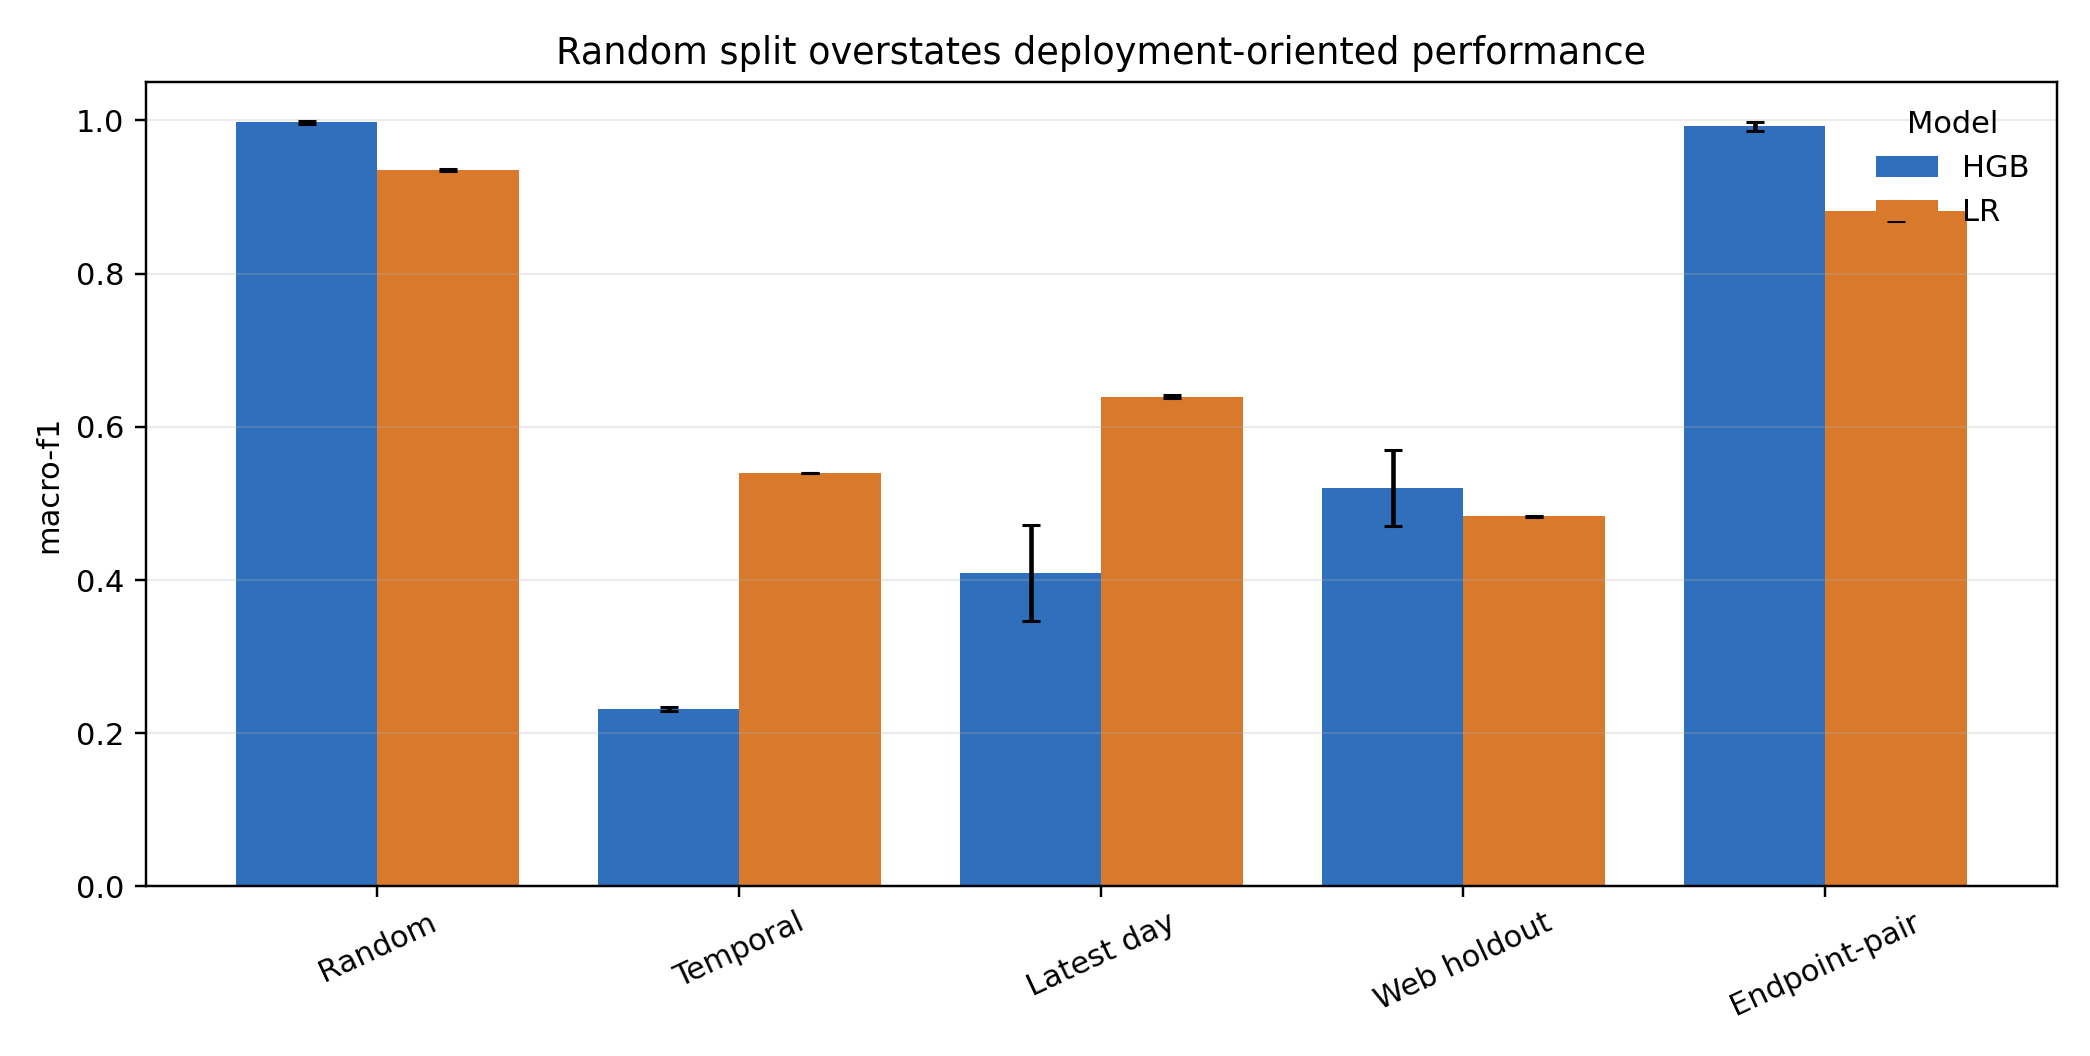
\includegraphics[width=\linewidth]{figures/core_random_vs_stress_macro_f1.png}
\caption{Full-data macro-F1 by split and model across seeds 42, 7 and 99. Bars show means over seeds and feature tiers; error bars show standard deviation over the same experimental units.}
\label{fig:core-split-gap}
\end{figure}

\subsection{Cyber Transferability Score}

We define a simple Cyber Transferability Score (CTS):
\[
\mathrm{CTS}(m,s)=\frac{\mathrm{macroF1}(m,s)}{\mathrm{macroF1}(m,\mathrm{random})},
\]
where \(m\) is the model and \(s\) is a stress-test split. Table~\ref{tab:cts} reports mean CTS across seeds.

CTS is a relative robustness measure. A raw stress-split macro-F1 reports absolute task performance, whereas CTS reports how much of the random-split performance survives under a deployment-oriented shift. This is useful because models can have different random-split ceilings: LR may look weaker than HGB under IID evaluation while retaining a larger fraction of its score under time or scenario shift. CTS is not a replacement for macro-F1; it is reported alongside absolute metrics to prevent a model with low random performance from appearing robust merely because its denominator is small.

\begin{table}[ht]
\centering
\caption{CTS macro-F1 mean and standard deviation across seeds.}
\label{tab:cts}
\begin{tabular}{llcc}
\toprule
Target split & Model & CTS mean & CTS std \\
\midrule
Endpoint-pair holdout & HGB & 0.9946 & 0.0048 \\
Temporal & HGB & 0.2321 & 0.0013 \\
Latest-day holdout & HGB & 0.4099 & 0.0341 \\
Scenario holdout Web & HGB & 0.5219 & 0.0387 \\
Endpoint-pair holdout & LR & 0.9426 & 0.0155 \\
Temporal & LR & 0.5772 & 0.0004 \\
Latest-day holdout & LR & 0.6834 & 0.0018 \\
Scenario holdout Web & LR & 0.5163 & 0.0004 \\
\bottomrule
\end{tabular}
\end{table}

These values quantify the main message: high random-split macro-F1 does not imply high transferability under time or scenario shifts.

\subsection{Paired robustness statistics}

Table~\ref{tab:paired-stats} reports paired stress-minus-random deltas and stress/random ratios. All stress splits are worse than the paired random baseline for both models. The exact sign-flip p-value is 0.0313 in every row because all six paired differences have the same sign; with six pairs this is the smallest possible two-sided value. Standardized effect sizes are not shown in the table because very low inter-seed variance can make them numerically unstable.

\begin{table}[ht]
\centering
\small
\caption{Paired random-vs-stress macro-F1 statistics across seeds and feature tiers. CI values are bootstrap 95\% intervals over six paired experimental units.}
\label{tab:paired-stats}
\begin{tabular}{llccc}
\toprule
Model & Stress split & Delta [95\% CI] & Ratio [95\% CI] & p \\
\midrule
HGB & Temporal & -0.7662 [-0.7674, -0.7650] & 0.2320 [0.2307, 0.2337] & 0.0313 \\
HGB & Latest-day & -0.5887 [-0.6281, -0.5486] & 0.4099 [0.3697, 0.4505] & 0.0313 \\
HGB & Web holdout & -0.4770 [-0.4996, -0.4353] & 0.5219 [0.4993, 0.5634] & 0.0313 \\
HGB & Endpoint-pair & -0.0054 [-0.0089, -0.0020] & 0.9946 [0.9906, 0.9980] & 0.0313 \\
LR & Temporal & -0.3956 [-0.3964, -0.3947] & 0.5772 [0.5767, 0.5777] & 0.0313 \\
LR & Latest-day & -0.2963 [-0.2980, -0.2947] & 0.6834 [0.6817, 0.6851] & 0.0313 \\
LR & Web holdout & -0.4526 [-0.4534, -0.4516] & 0.5163 [0.5157, 0.5170] & 0.0313 \\
LR & Endpoint-pair & -0.0537 [-0.0632, -0.0443] & 0.9426 [0.9325, 0.9527] & 0.0313 \\
\bottomrule
\end{tabular}
\end{table}

\subsection{Binary calibration under stress}

The seed-42 advanced run provides binary calibration metrics for the \texttt{deployment\_safe} tier. Table~\ref{tab:binary-calibration} shows macro-F1 and ECE. The hardest shifts are not only lower-performing; they are poorly calibrated.

\begin{table}[ht]
\centering
\caption{Seed-42 binary macro-F1 and ECE for the \texttt{deployment\_safe} feature tier.}
\label{tab:binary-calibration}
\begin{tabular}{llcc}
\toprule
Model & Split & Macro-F1 & ECE \\
\midrule
HGB & Random stratified & 0.9960 & 0.0009 \\
LR & Random stratified & 0.9370 & 0.0345 \\
HGB & Temporal & 0.2296 & 0.7013 \\
LR & Temporal & 0.5395 & 0.3955 \\
HGB & Latest-day holdout & 0.3678 & 0.4180 \\
LR & Latest-day holdout & 0.6370 & 0.2528 \\
HGB & Scenario holdout Web & 0.6218 & 0.0093 \\
LR & Scenario holdout Web & 0.4833 & 0.0661 \\
HGB & Endpoint-pair holdout & 0.9917 & 0.0020 \\
LR & Endpoint-pair holdout & 0.8837 & 0.0584 \\
\bottomrule
\end{tabular}
\end{table}

Temporal ECE reaches 0.7013 for HGB and 0.3955 for LR, suggesting severe overconfidence or miscalibration under shift.

\subsection{External validation on CSE-CIC-IDS2018}

Table~\ref{tab:external-cse} reports the binary external validation on the 363,648-row CSE-CIC-IDS2018 stratified sample. The same qualitative concern appears outside the local CICIDS2017-like CSV files: random-split scores are much higher than temporal-holdout scores for all three tested models.

\begin{table}[ht]
\centering
\caption{External validation on real CSE-CIC-IDS2018 CSVs. Macro-F1 on the 363,648-row stratified validation sample from all 10 processed CSV files.}
\label{tab:external-cse}
\begin{tabular}{lcccc}
\toprule
Model & Random & Temporal & Latest-day & Web holdout \\
\midrule
LR & 0.8425 & 0.3913 & 0.4787 & 0.5522 \\
HGB & 0.9362 & 0.1037 & 0.8070 & 0.7161 \\
RF & 0.9195 & 0.1050 & 0.8739 & 0.5779 \\
\bottomrule
\end{tabular}
\end{table}

The external latest-day result is deliberately not over-interpreted: RF remains strong on that split even though it collapses under temporal holdout. This reinforces the paper's central claim that deployment reliability is split-specific and cannot be inferred from one favorable protocol. Post-hoc calibration was additionally evaluated on an earlier 200,928-row CSE-CIC sample and is split-dependent. For LR, isotonic calibration reduces random-split ECE from 0.0395 to 0.0040 and temporal ECE from 0.3619 to 0.1533, but Web-holdout ECE worsens from 0.1693 to 0.2309. For HGB, isotonic calibration reduces random ECE from 0.0151 to 0.0029, but temporal ECE worsens from 0.0864 to 0.1310. Open-set scoring on a 50,000-row external subsample shows that Local Outlier Factor is much stronger than Isolation Forest for Web, Botnet and BruteForce unknown-family scoring, with AUROC values of 0.8990, 0.9574 and 0.9087 respectively. These results strengthen the conclusion that calibration and open-set behavior must be evaluated under each shift rather than assumed from random-split performance.

\subsection{Multiclass collapse under shifted splits}

Table~\ref{tab:multiclass} reports seed-42 multiclass macro-F1 and weighted-F1. Weighted-F1 can remain high even when macro-F1 collapses, especially in scenario and endpoint holdouts. This confirms that weighted aggregate metrics mask minority-class failures.

\begin{table}[ht]
\centering
\caption{Seed-42 multiclass results for the \texttt{deployment\_safe} feature tier.}
\label{tab:multiclass}
\begin{tabular}{llcc}
\toprule
Model & Split & Macro-F1 & Weighted-F1 \\
\midrule
HGB & Random stratified & 0.7479 & 0.9901 \\
LR & Random stratified & 0.4487 & 0.9175 \\
HGB & Temporal & 0.0415 & 0.1360 \\
LR & Temporal & 0.0453 & 0.1621 \\
HGB & Latest-day holdout & 0.0523 & 0.4256 \\
LR & Latest-day holdout & 0.0546 & 0.4439 \\
HGB & Scenario holdout Web & 0.0762 & 0.9791 \\
LR & Scenario holdout Web & 0.0667 & 0.9225 \\
HGB & Endpoint-pair holdout & 0.4447 & 0.9923 \\
LR & Endpoint-pair holdout & 0.3044 & 0.9051 \\
\bottomrule
\end{tabular}
\end{table}

The Azure log emitted 16 sklearn warnings stating that predicted labels contained classes absent from the true labels during shifted multiclass/per-class evaluation. This is not a cosmetic warning; it indicates label-support shift and should be discussed as part of the failure mode.

\begin{figure}[ht]
\centering
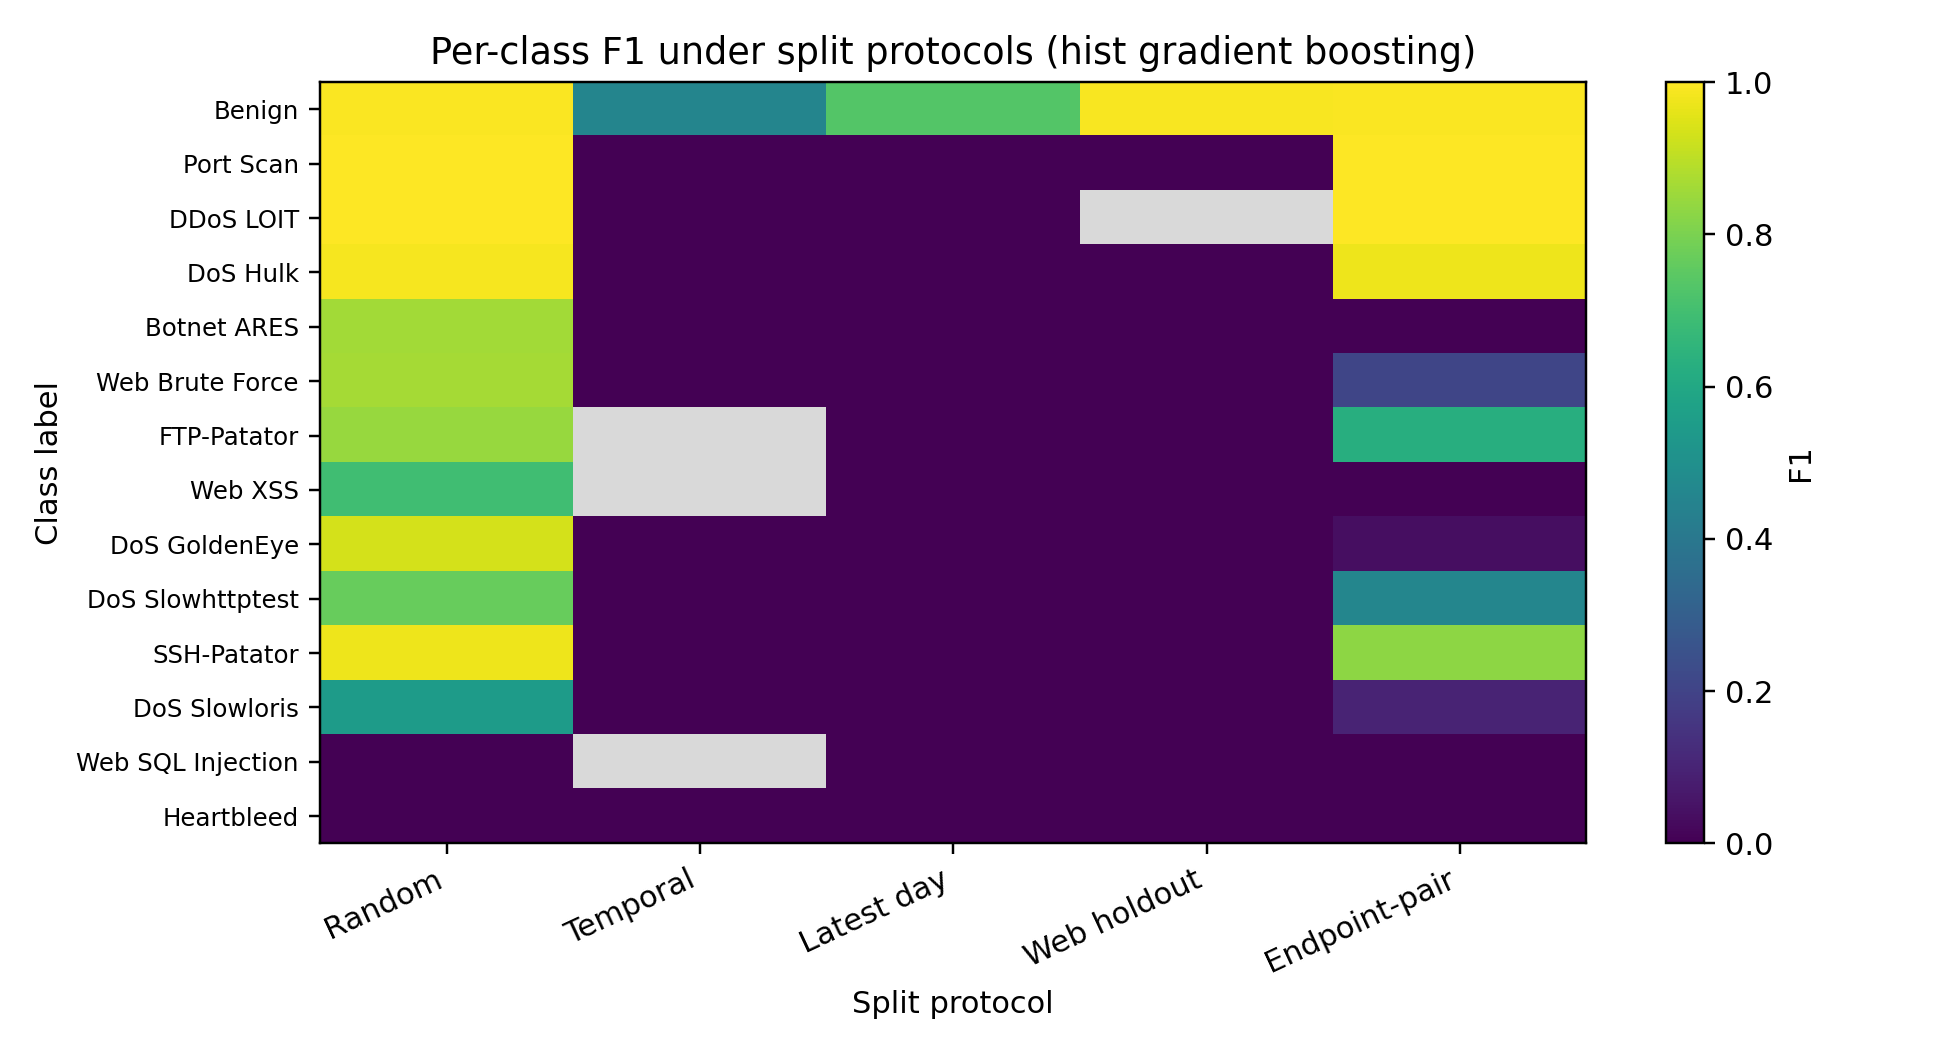
\includegraphics[width=\linewidth]{figures/per_class_f1_heatmap_hgb.png}
\caption{HGB per-class F1 across split protocols for the seed-42 advanced run. Gray cells indicate classes absent from the corresponding test split.}
\label{fig:per-class-heatmap}
\end{figure}

\subsection{Rare-class behavior}

Rare-class results further expose the weakness of global metrics. In Web scenario holdout, all three Web rare classes have F1 equal to 0.0 for both LR and HGB despite nonzero test support. Table~\ref{tab:rare-web} reports the verified values.

\begin{table}[ht]
\centering
\caption{Rare Web-class F1 under Web scenario holdout.}
\label{tab:rare-web}
\begin{tabular}{lccc}
\toprule
Label & Support & LR F1 & HGB F1 \\
\midrule
Web Brute Force & 2734 & 0.0000 & 0.0000 \\
Web SQL Injection & 24 & 0.0000 & 0.0000 \\
Web XSS & 1358 & 0.0000 & 0.0000 \\
\bottomrule
\end{tabular}
\end{table}

This result should be framed as a controlled failure analysis. It does not show that the models solve rare attack detection; it shows that random or weighted metrics can hide rare-class failure.

\subsection{Open-set unknown-family holdout}

Table~\ref{tab:openset} reports unknown-family uncertainty metrics. Uncertainty behavior is model- and family-dependent. HGB uncertainty ranks unknown traffic well for all four families, whereas LR fails badly for DDoS uncertainty ranking despite high binary attack recall.

\begin{table}[ht]
\centering
\caption{Seed-42 open-set unknown-family results.}
\label{tab:openset}
\begin{tabular}{llccc}
\toprule
Unknown family & Model & Support & Uncertainty AUROC & Unknown recall at p90 \\
\midrule
Web & LR & 4116 & 0.8697 & 0.0649 \\
Web & HGB & 4116 & 0.9353 & 0.6618 \\
Botnet & LR & 5508 & 0.7607 & 0.0005 \\
Botnet & HGB & 5508 & 0.9262 & 0.6899 \\
PortScan & LR & 161323 & 0.9501 & 0.2348 \\
PortScan & HGB & 161323 & 0.9954 & 0.4393 \\
DDoS & LR & 95733 & 0.2019 & 0.0545 \\
DDoS & HGB & 95733 & 0.9587 & 0.3570 \\
\bottomrule
\end{tabular}
\end{table}

This is a diagnostic baseline rather than a complete open-set method. A stronger final paper should add anomaly or open-set baselines.

\subsection{Abstention and selective prediction}

At approximately 90\% coverage, selective macro-F1 remains poor on hard shifts. For example, HGB temporal selective macro-F1 is 0.2416 and accepted attack recall is 0.0000; LR temporal selective macro-F1 is 0.5931 with accepted attack recall 0.3975. At 50\% coverage, LR improves on temporal and latest-day holdouts, but this requires sending half of the flows to review. The practical interpretation is therefore a coverage-risk tradeoff, not an automatic model improvement.

\subsection{Explanation stability}

Top-15 explanation-overlap Jaccard against the random-stratified baseline is much lower for HGB than LR under the hardest shifts. HGB temporal Jaccard is 0.0714, corresponding to only two overlapping top-15 features, whereas LR temporal Jaccard is 0.5789. This suggests that HGB feature importance is more sensitive to split protocol. However, the current HGB permutation importance uses a sample size of 2000 and one repeat; a final journal version should increase repeats and add uncertainty estimates.

\subsection{Practical SOC guidance}

Table~\ref{tab:soc-guidance} summarizes the operational guidance implied by the experiments. The table is intentionally conservative: it does not recommend deploying a model solely because its random-split score is high.

\begin{table}[ht]
\centering
\small
\caption{Practical guidance for SOC-oriented use of the evaluated protocol.}
\label{tab:soc-guidance}
\begin{tabular}{
>{\raggedright\arraybackslash}p{0.24\linewidth}
>{\raggedright\arraybackslash}p{0.28\linewidth}
>{\raggedright\arraybackslash}p{0.38\linewidth}}
\toprule
Decision point & Recommendation & Rationale \\
\midrule
Model selection & Do not rank models using random split only. & HGB dominates random macro-F1 but collapses under temporal holdout; LR is less impressive under random split but more stable for some shifts. \\
Validation protocol & Require temporal and scenario holdouts before deployment claims. & These splits expose failures hidden by random stratification and weighted metrics. \\
Alert triage & Use calibration and abstention only after split-specific validation. & Calibration helps in some random/external cases but can worsen ECE under stress splits. \\
Rare attacks & Inspect per-class and rare-class F1, not only binary metrics. & Web rare classes reach F1=0 under Web holdout despite acceptable aggregate scores. \\
Operational reporting & Report CTS, absolute macro-F1, calibration and review burden together. & A single metric cannot capture accuracy, transferability, confidence quality and analyst workload. \\
\bottomrule
\end{tabular}
\end{table}

\section{Discussion}

The results support three conclusions.

First, random-split benchmark accuracy is not a reliable proxy for deployment reliability. HGB appears nearly perfect under random stratification, but its temporal macro-F1 and calibration collapse. LR is less impressive under random stratification but can be more stable under some shifts.

The likely explanation is that HGB exploits sharper split-specific feature interactions. That behavior is useful under IID evaluation but brittle under chronological shift: HGB temporal macro-F1 drops to 0.2315 and its top-15 explanation overlap with the random baseline is only 0.0714. LR has lower random-split macro-F1 but higher temporal macro-F1 and a higher explanation-overlap Jaccard of 0.5789. This does not make LR universally better; it shows that model ranking depends on the deployment stressor.

Second, binary evaluation is insufficient. Multiclass macro-F1, rare-class results and Web holdout results reveal failures that are hidden by weighted or binary metrics. This is particularly important for SOC deployment, where missing a rare but critical attack can be operationally unacceptable. The heatmap in Figure~\ref{fig:per-class-heatmap} makes the same point visually: several attack families that look strong under random stratification become near-zero under temporal, latest-day or Web holdout evaluation.

Third, uncertainty and explanations are not automatically robust. Open-set results vary strongly by model and unknown family, while explanation stability changes across split protocols. These behaviors should be evaluated as first-class outcomes, not as optional post-hoc figures.

\section{Threats to Validity}

\paragraph{Internal validity.}
The pipeline records dataset hashes, feature hashes, split hashes and Azure ML provenance, but implementation bugs remain possible. We mitigate this risk through unit tests, tracked artifacts and explicit logging of failures such as the initial OOM run and LR convergence warnings. The endpoint-pair split is also a possible internal-validity concern because it is much less discriminating than temporal and scenario holdouts; this may reflect genuine robustness for endpoint-pair grouping, or a grouping definition that is too granular to simulate deployment shift.

\paragraph{External validity.}
The main evidence still comes from one CICIDS2017-like dataset. The CSE-CIC-IDS2018 result uses all 10 public processed CSV files for the raw audit and a 363,648-row stratified real-data sample for experiments, but it is still not a full cross-dataset benchmark over original class priors. The paper should therefore claim external consistency evidence, not universal generalization. Prior studies also report CICIDS2017 flow-construction and labelling issues. These issues motivate the study but limit claims about real-world attack detection.

\paragraph{Construct validity.}
The study uses macro-F1, CTS, calibration error, selective prediction and explanation overlap as deployment-reliability proxies. These metrics capture important failure modes but do not fully encode SOC cost, alert fatigue, incident criticality or analyst workflow. The practical guidance should therefore be interpreted as evaluation guidance, not as a deployment certification.

\paragraph{Conclusion validity.}
The binary core is validated on seeds 42, 7 and 99, and the paired random-vs-stress statistics use the six available seed-by-feature-tier units. The advanced analyses are currently available for seeds 42 and 99, with seed 7 still running at the time of this draft. Final claims about rare-class, open-set, calibration and explanation stability should be repeated on all three seeds if compute budget allows. LR convergence is fixed for seed 42 with \texttt{max\_iter=2000}; corrected LR2000 reruns without the timestamp-derived \texttt{hour} feature have been submitted for seeds 42, 7 and 99, but their artifacts were not yet available at the time of this draft.

\paragraph{Open-set baseline strength.}
The main advanced open-set analysis uses classifier uncertainty. The external validation adds Isolation Forest and Local Outlier Factor, and separate full-data Isolation Forest jobs are completed for seeds 42 and 99. These are still baseline anomaly detectors, and seed 7 remains queued. A final version should compare additional open-set or anomaly approaches if scope permits.

\paragraph{Explanation precision.}
HGB explanation stability uses lightweight permutation importance. A final version should use more repeats and confidence intervals.

\section{Conclusion}

FAIR-ML-CYBER shows that CICIDS2017-like evidence can support a meaningful Q1-oriented contribution if the paper is framed as a rigorous evaluation and benchmark-validity study, and if its limits are tested against external data. The verified results show that random-split scores are overly optimistic, temporal and scenario shifts expose major transferability failures, calibration degrades under shift, rare classes are poorly detected, open-set behavior is inconsistent and explanation stability depends on the split protocol. The CSE-CIC-IDS2018 validation supports the same caution: random-split performance remains insufficient evidence of deployment reliability.

The manuscript should not claim a new state-of-the-art detector. Its strongest claim is methodological: NIDS evaluation must include leakage-aware stress tests, transferability metrics, rare-class analysis, calibration, abstention, open-set diagnostics and explanation stability before benchmark scores can be interpreted as deployment evidence.

\section*{Reproducibility Statement}

The repository records Azure ML job names, Git commits, dataset hashes, feature hashes, split hashes, runtimes and evidence snapshots. The main verified artifacts are:
\begin{itemize}[leftmargin=*]
  \item \texttt{evidence/fullcore-mem-s42-001/}
  \item \texttt{evidence/fullcore-mem-s7-001/}
  \item \texttt{evidence/fullcore-mem-s99-001/}
  \item \texttt{evidence/fullcore-lr2000-s42-001/}
  \item \texttt{evidence/q1-stats-fullcore-multiseed-001/}
  \item \texttt{evidence/advanced-core-s42-001/}
  \item \texttt{evidence/advanced-core-s99-001/}
  \item \texttt{evidence/cse-cic-ids2018-partial-s42-001/}
  \item \texttt{evidence/cse-cic-ids2018-full-sample-s42-001/}
  \item \texttt{evidence/open-set-if-s42-001/}
  \item \texttt{evidence/open-set-if-s99-001/}
\end{itemize}

\bibliographystyle{plain}
\bibliography{../references}

\end{document}
